%
%
\subsection{NASA Rotor 37}
\label{nasa_rotor37.subsec}
%
 A low-aspect-ratio transonic inlet rotor for a core compressor,
 designated NASA rotor 37, was used in the present section to validate
 the steady state code for three-dimensional geometries.
 The rotor was originally designed and tested at NASA Lewis Research
 Center by Reid and Moore \citeyear{Reid:1}.
 In the CFD assessment, the rotor was tested in isolation by several
 researchers (Suder and Celestina \citeyearNP{Suder:1},
 Chima \citeyearNP{Chima:2}, Arima et al. \citeyearNP{Arima:1}).
 The rotor geometry together with the location measured using
 aerodynamics probes and laser anemometer measurements
 are shown in Fig. \ref{rot37_geo.fig}.
%
\begin{figure}
  \begin{center}
   \begin{tabular}{c}
    \subfigure
      {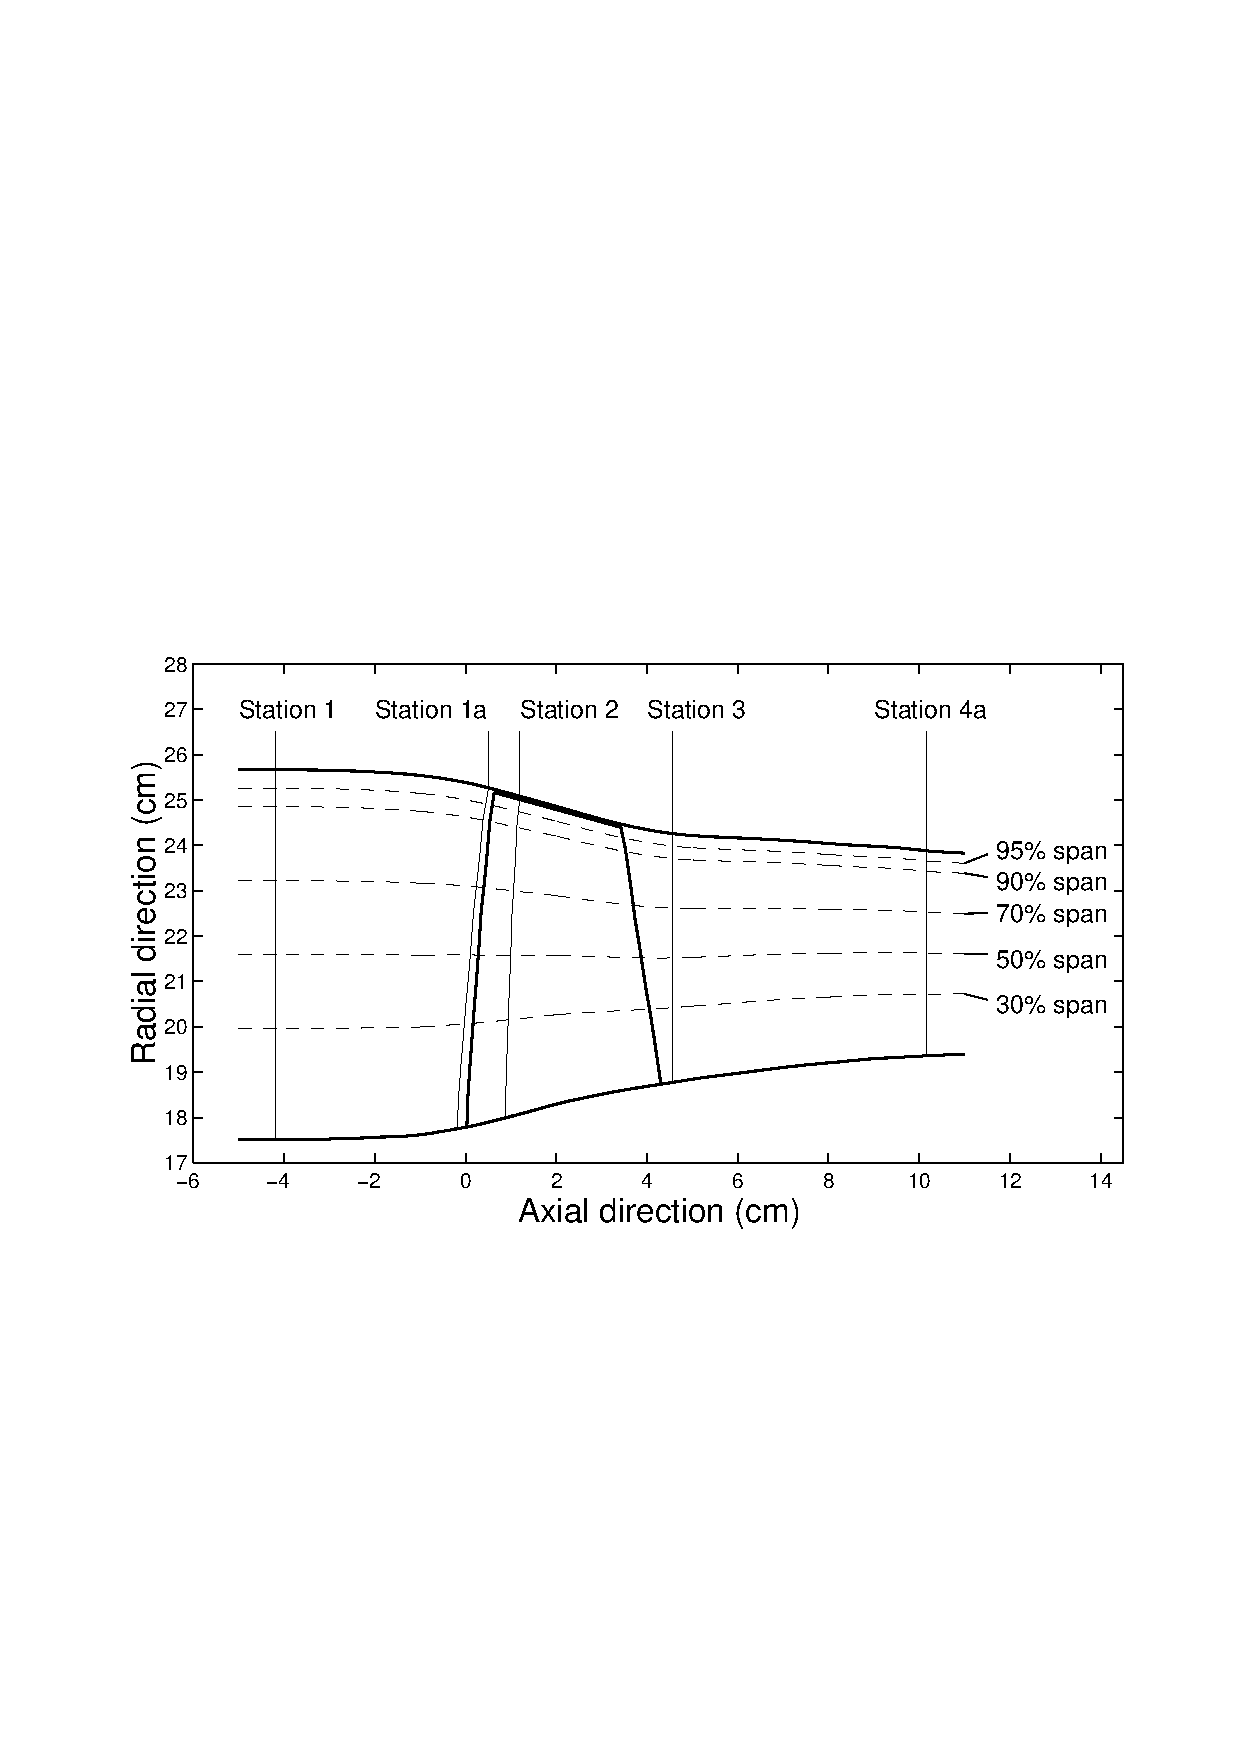
\includegraphics[width=100mm,clip=t]{CHAP_NONLIN/FIGURE/rotgeo.pdf}}
      \vspace{-4mm}\\
    \subfigure
      {\begin{tabular}{|c|c|c|c|c|c|}\hline
        Station & 1 & 1a & 2 & 3 & 4a \\ \hline
        x (cm) & -4.19 & $-5\%$ chord & $20\%$ chord & 4.57 & 10.16 \\ \hline
      \end{tabular}}
   \end{tabular}
  \end{center}
  \vspace{-8mm}
  \caption{NASA Rotor 37: $x-r$ view showing locations at which data were
           acquired}
  \label{rot37_geo.fig}
\end{figure}
%

 The rotor has a design pressure ratio of 2.106 at a mass flow of
 $20.19\ kg/s$, with a measured chocking mass flow of $20.93\ kg/s$.
 The rotor has 36 multiple-circular-arc blades with a hub-tip ratio
 of 0.7, an aspect ratio of 1.19, and a tip solidity
 of 1.288. The running tip clearance was estimated to be $0.356\ mm$
 ($0.45\%$ span). The design wheel speed is $17,188.7\ rpm$
 giving a nominal tip speed of $454\ m/s$.
 A brief description of the test facility and laser anemometer
 system is given by Suder and Celestina \citeyear{Suder:1}.

%
\begin{figure}
 \begin{center}
  \begin{tabular}{cc}
    \subfigure[Frontal view]
       {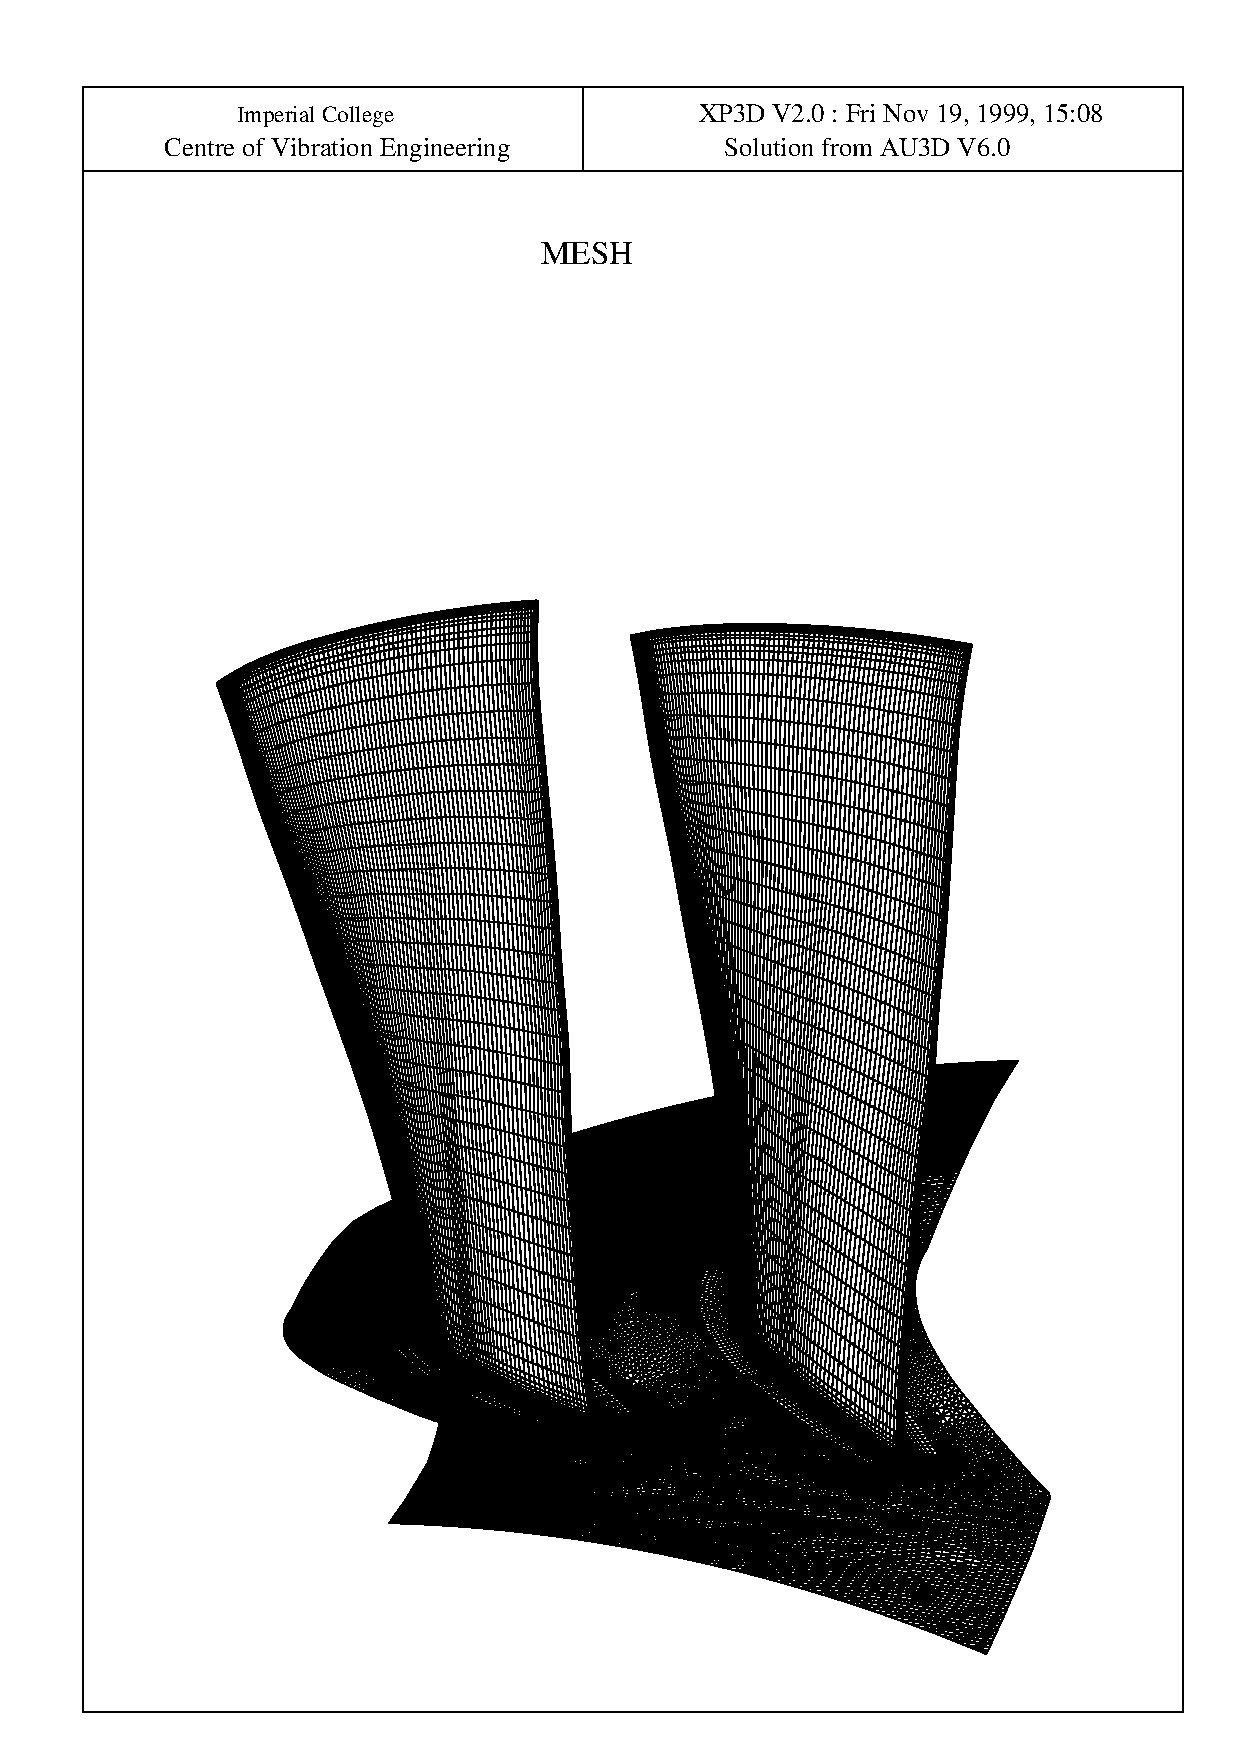
\includegraphics[width=55mm,clip=t]{CHAP_NONLIN/FIGURE/rot37_mesh1.pdf}}
        &
    \subfigure[$x-r\theta$ view]
       {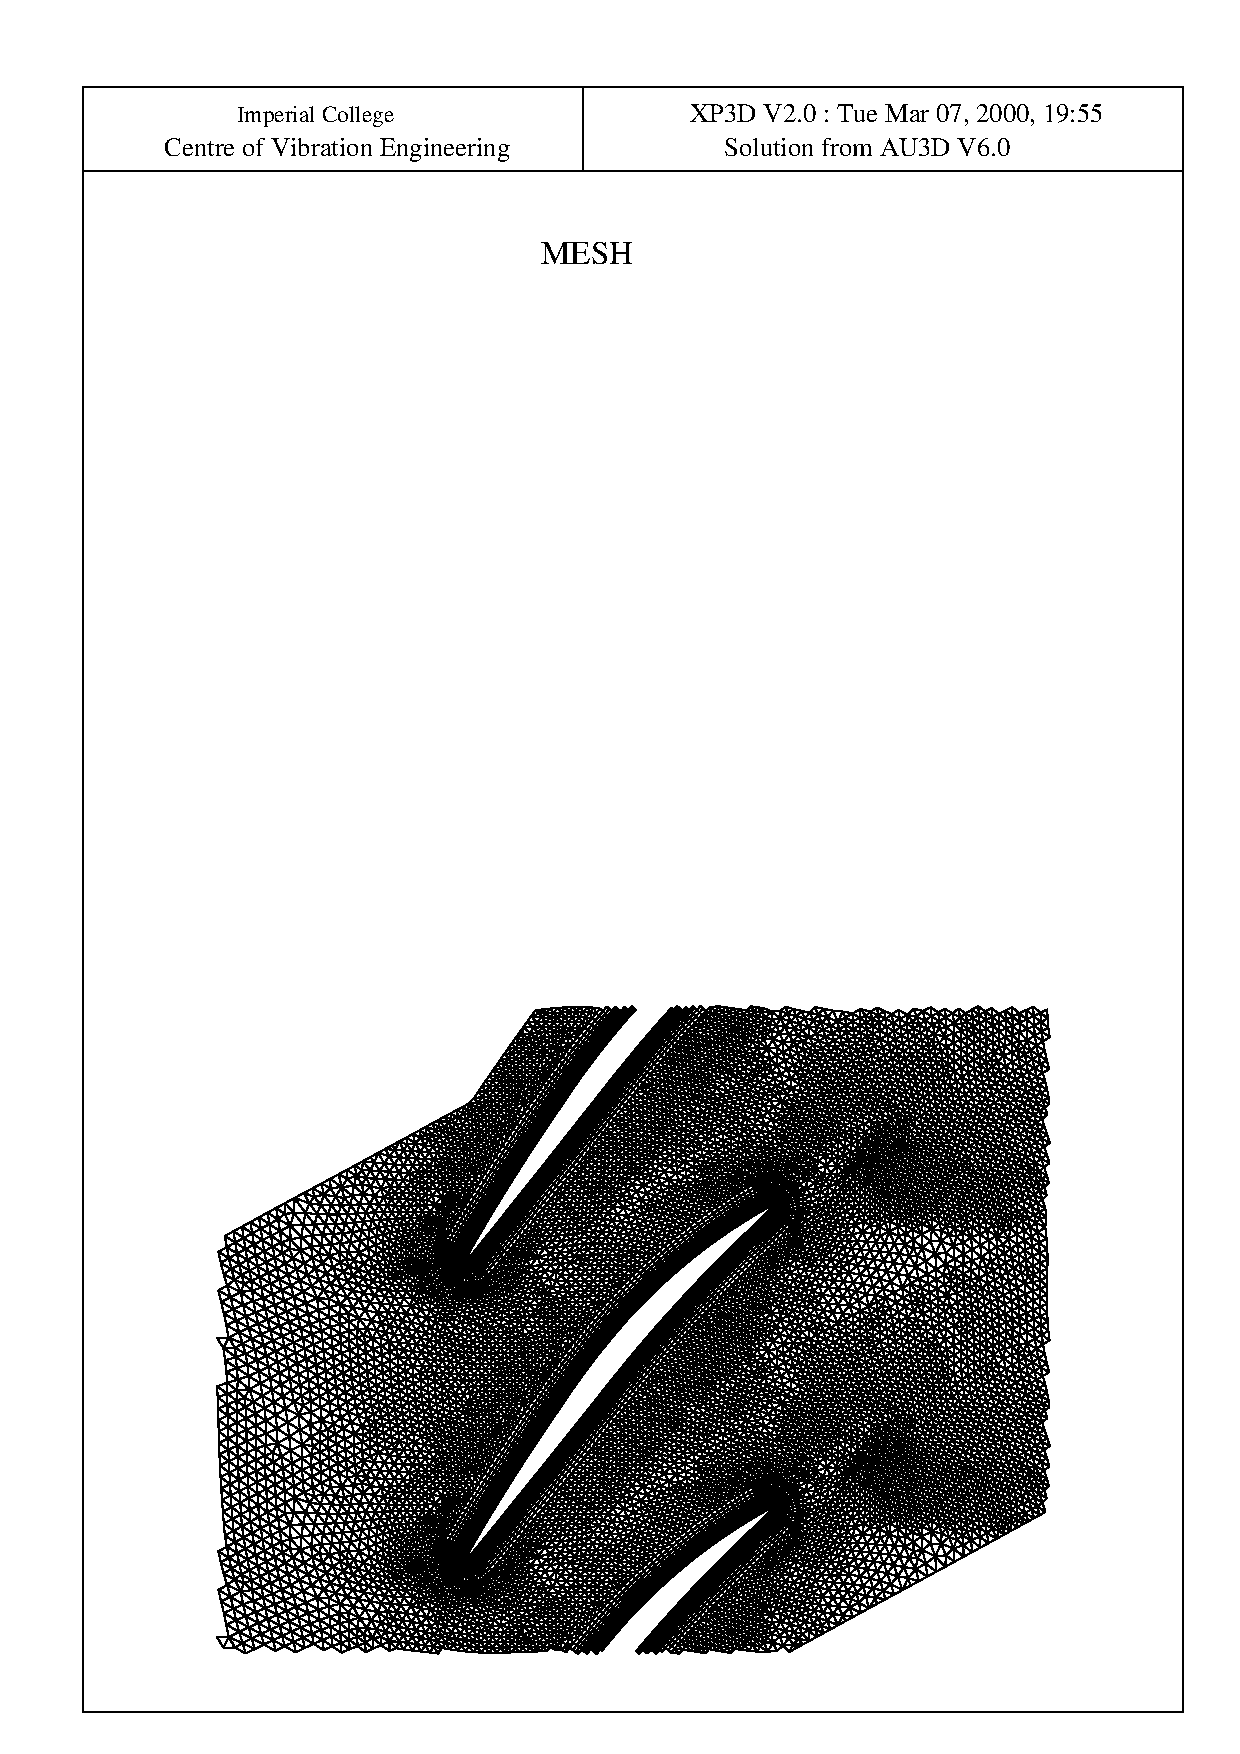
\includegraphics[width=85mm,clip=t]{CHAP_NONLIN/FIGURE/rot37_mesh4.pdf}}
      \vspace{-4mm}\\
    \subfigure[Tip gap view]
       {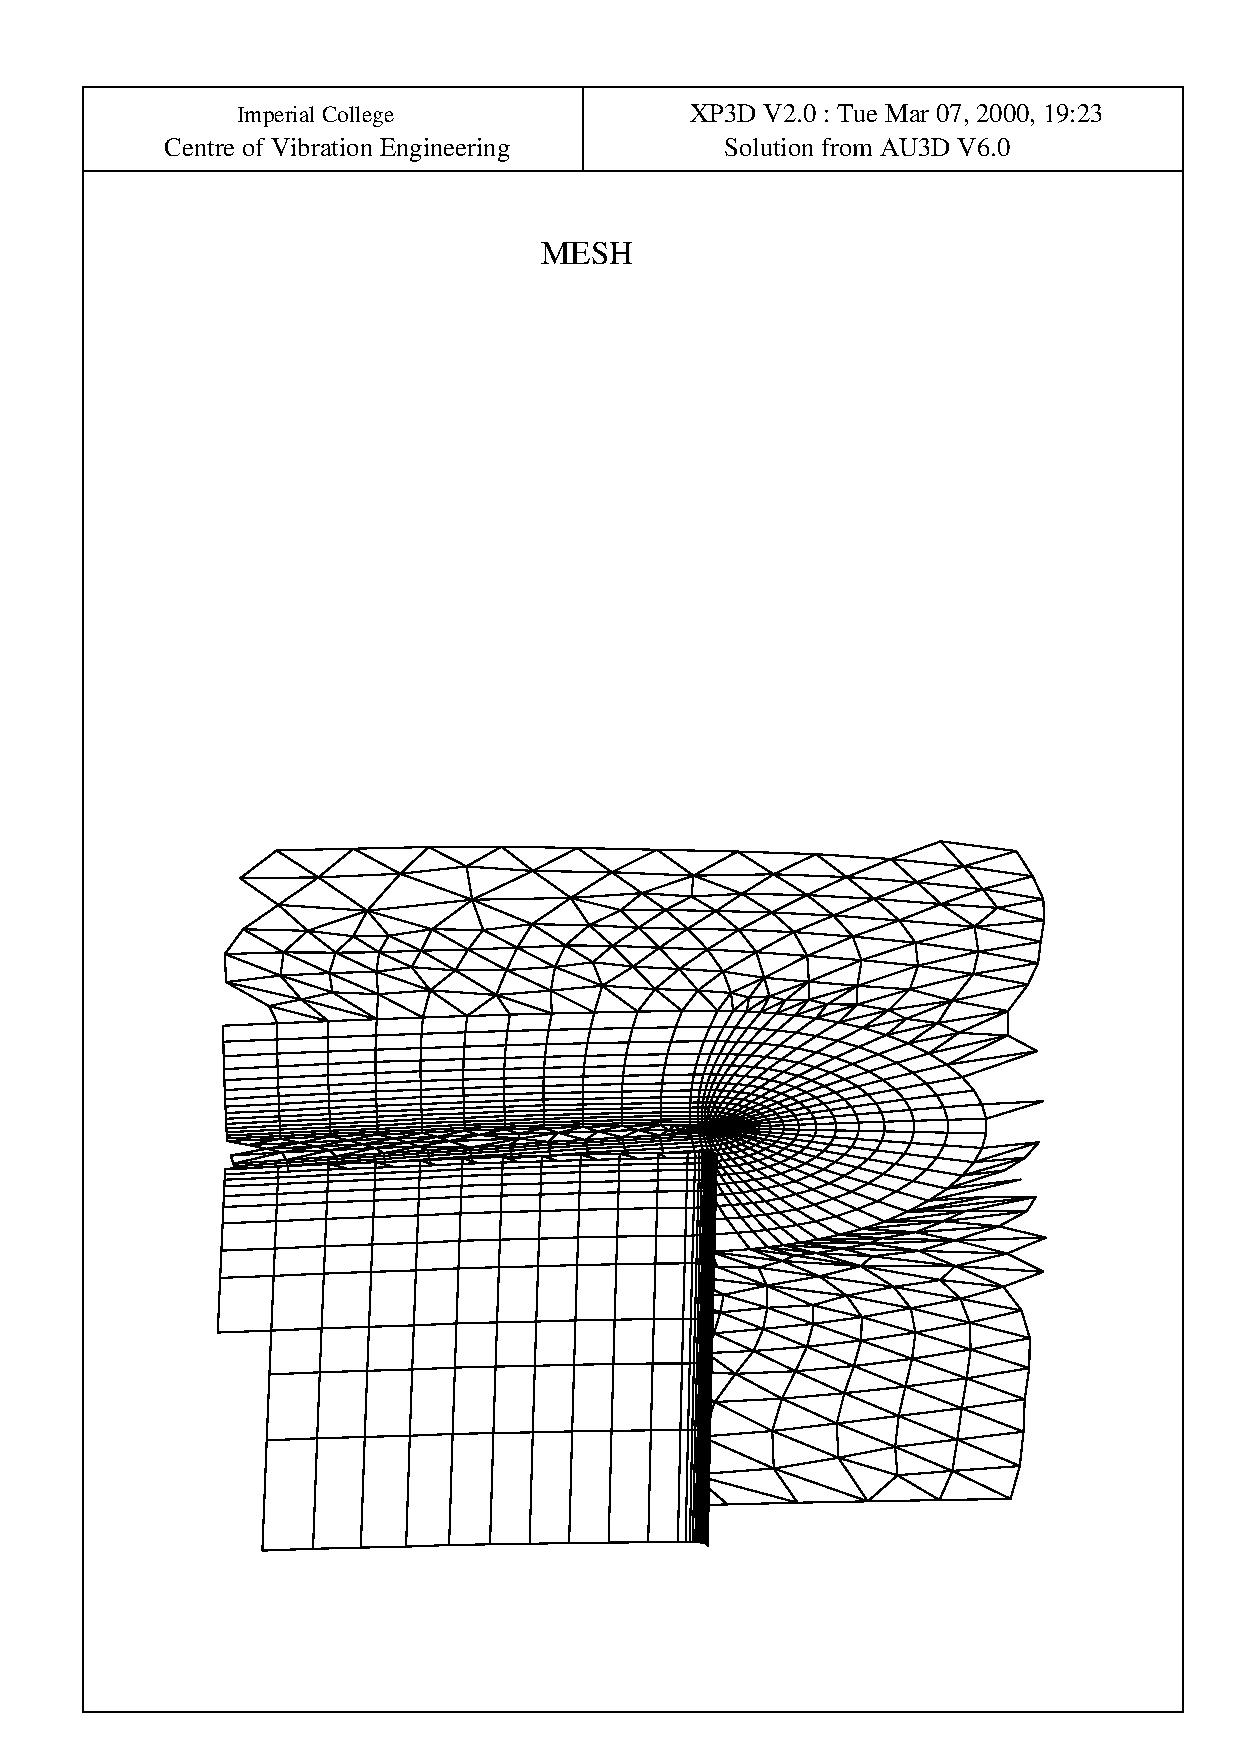
\includegraphics[width=55mm,clip=t]{CHAP_NONLIN/FIGURE/rot37_mesh3.pdf}}
        &
    \subfigure[$x-r$ view]
       {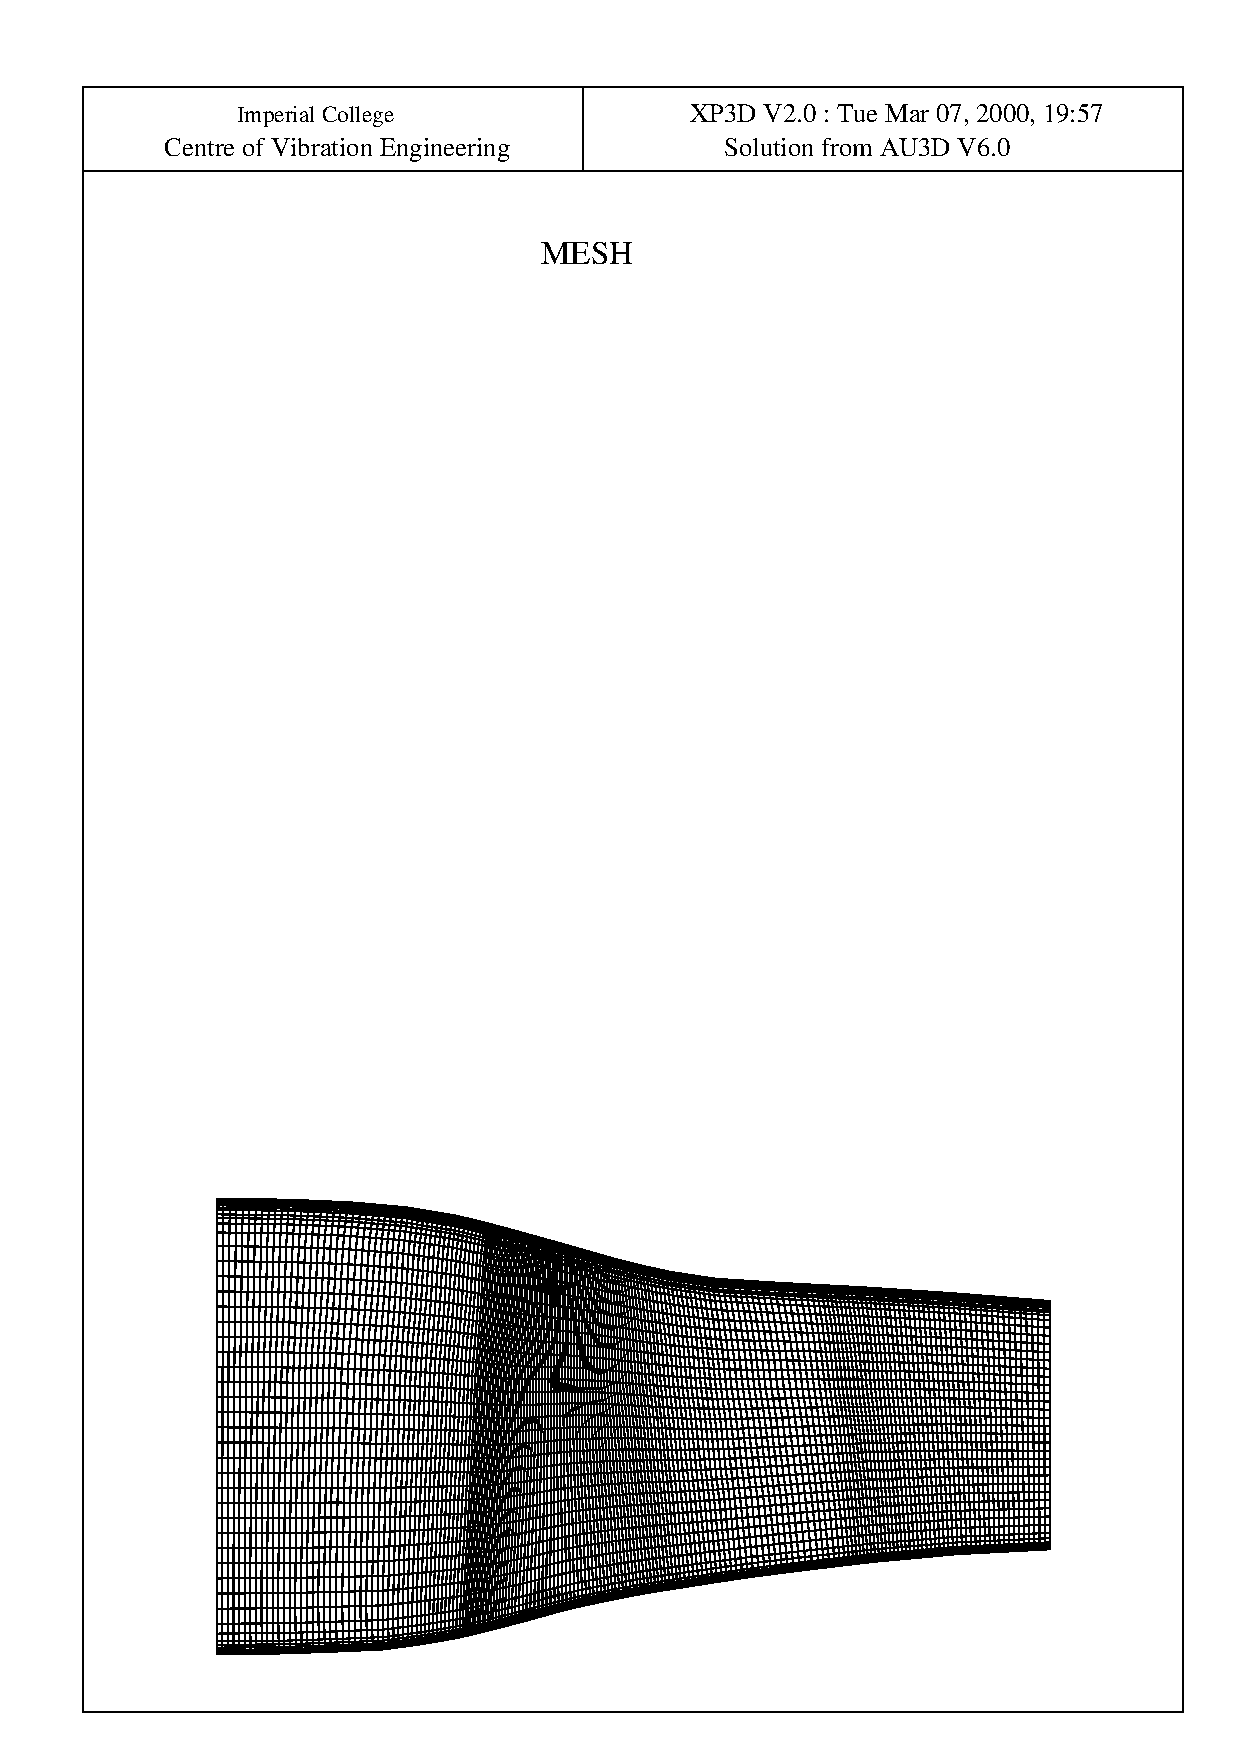
\includegraphics[width=85mm,clip=t]{CHAP_NONLIN/FIGURE/rot37_mesh2.pdf}}
  \end{tabular}
 \end{center}
 \vspace{-8mm}
 \caption{NASA Rotor 37: computational mesh}
 \label{rot37_mesh.fig}
\end{figure}
%
 Views of the computational mesh,
 generated with the semi-structured mesh generator
 LEVMAP described in chapter \ref{mesh.chap}
 (Sbardella et al. \citeyearNP{Luca:9}),
 are shown in Fig. \ref{rot37_mesh.fig}.
 The computational domain extends axially from station 1 in Fig.
 \ref{rot37_geo.fig} up to $x=10.67\ cm$ which corresponds to
 station 4 (not shown in Fig. \ref{rot37_geo.fig}). It contains 174,900 hexahedra
 in the boundary layer reagion and 607,067 wedges in the rest of the domain for
 a total number of point of 504,946. The boundary layer mesh does not resolve
 the viscous sublayer thus calculations with wall-slip condition
 (\ref{flow_tangency1.eq}) and wall-shear
 stresses evaluated using the low of the wall are considered here.
 As shown in Fig. \ref{rot37_geo.fig}c, the tip clearance flows will be modelled
 in a straightforward way by simply meshing the gap and setting the rotation
 speed at the casing to zero.
 At the hub section the reagion $x < -0.264\ cm$, $x > 4.521\ cm$,
 is not rotating so the rotational speed is also set to zero.
%
\begin{figure}
 \begin{center}
  \begin{tabular}{cc}
    \subfigure[$95\%$ span]
       {\includegraphics[width=60mm,clip=t]{FIGURE/CHAP2/rot37_cont_95.pdf}}
        &
    \subfigure[$97\%$ span]
       {\includegraphics[width=60mm,clip=t]{FIGURE/CHAP2/rot37_cont_97.pdf}}
       \vspace{-4mm} \\
    \subfigure[$99\%$ span]
       {\includegraphics[width=60mm,clip=t]{FIGURE/CHAP2/rot37_cont_99.pdf}}
        &
    \subfigure[Tip gap]
       {\includegraphics[width=60mm,clip=t]{FIGURE/CHAP2/rot37_cont_gap.pdf}}
  \end{tabular}
 \end{center}
 \vspace{-8mm}
 \caption{Rotor 37: Mach number contours}
 \label{rot37_mach.fig}
\end{figure}
%
